\documentclass{article}
\usepackage[UKenglish]{babel}
\usepackage[UKenglish]{isodate}
\usepackage[utf8]{inputenc}
\usepackage{fullpage}
\usepackage{amsmath}
\usepackage{amsthm}
\usepackage{mathrsfs}
\usepackage{oz}
\usepackage[linesnumbered,ruled,vlined]{algorithm2e}
\usepackage{tikz}
\usepackage[capitalize]{cleveref}

\usetikzlibrary{arrows,fit,positioning,trees}

\theoremstyle{definition}
\newtheorem{definition}{Definition}
\newtheorem{example}{Example}

\DeclareMathOperator{\Imm}{Im}
\DeclareMathOperator{\Doms}{Doms}
\DeclareMathOperator{\Vars}{Vars}
\DeclareMathOperator{\WMC}{WMC}

\title{Empowering Domain Recursion in Symmetric Weighted First-Order Model Counting}

\begin{document}
\maketitle

\section{Basic Definitions}
% TODO (later): maybe mathcal instead of mathscr

\paragraph{Things I might need to explain.}
\begin{itemize}
\item notation: $\Imm$
\item atom
\item inequality constraint
\item $\Vars$, $\Vars(c) = \Vars(P) \cup \Vars(N) \cup \Vars(C)$
\item $\Doms$ on both formulas and clauses. $\Doms(c) = \Imm \delta_c$, and $\Doms(\phi) = \bigcup_{c \in \phi} \Doms(c)$.
\item the hash codes of clauses and formulas. Introduce the $\#$ notation.
\item substitution
\item (strict) equality of clauses. It's important to mention that we check the number of variables but not their domains.
\item size of a domain, how each domain is partitioned into two, and how we iterate over all possible integer partitions of length two.
\item maybe: notation for partial function, notation for powerset
\item notation for projection (or avoid it?)
\item $\WMC$
\end{itemize}

Let $\mathscr{V}$ be the set of circuit nodes.

TODO: merge $\kappa$ and $\iota$ into one.

TODO: maybe $\pi$ and $\kappa$ are global enough to have more unique names.

\begin{definition}
  A \emph{domain} is a set with elements not used anywhere else.\footnote{In the context of functions, the domain of a function $f$ retains its usual meaning and is denoted $\dom(f)$.} Let $\mathscr{D}$ be the set of all domains (note that this set expands during compilation).

  We now define two partial maps $\pi$ and $\kappa$ with the same domain $\dom(\pi) = \dom(\kappa) \subset \mathscr{D}$. First, let $\pi\colon \mathscr{D} \pfun \mathscr{D}$ be a partial endomorphism on $\mathscr{D}$ that denotes the \emph{parent} relation, i.e., if $\pi(d) = e$ for some $d, e \in \mathscr{D}$, then we call $e$ the parent (domain) of $d$, and $e$ a child of $d$. Intuitively, $\pi$ arranges all domains into a forest---thus, we often use graph theoretical terminology to describe properties of and relationships between domains. Second, let $\kappa\colon \mathscr{D} \pfun \mathscr{V}$ be a partial map that assigns a \emph{cause node} to all non-root domains. Third, let $\iota\colon \mathscr{D} \pfun \{\, 0, 1 \,\}$ unambiguously order the children of any internal node, i.e., $\iota(d) \ne \iota(e)$ whenever $\pi(d) = \pi(e)$ for any $d, e \in \mathscr{D}$.\footnote{Here, each internal node has at most two children.}
\end{definition}

\begin{definition}
  A \emph{clause} is a triple $c = (P, N, C, \delta_c)$, where $P$ and $N$ are sets of atoms interpreted as positive and negative literals respectively, $C$ is a set of inequality constraints, and $\delta_c\colon \Vars(c) \to \mathscr{D}$ is a function that maps all variables in $c$ to their domains. Two clauses $c$ and $d = (P', N', C', \delta_d)$ are \emph{equivalent} (written $c \equiv d$) if there is a bijection $\beta\colon \Vars(c) \to \Vars(d)$ such that $c\beta = d\beta$. TODO: we will always use this subscript notation for the $\delta$'s.
\end{definition}

A \emph{formula} is a set of clauses.

\section{Identifying Possibilities for Recursion}

%% For succinctness, let $\mathscr{S} = \mathscr{D} \times \mathscr{D} \times 2^{\mathscr{V} \times \{\, 0, 1 \,\}}$.

%% Let $\nu\colon \mathscr{S} \to 2^{\mathscr{S}}$ be a map defined as
%% \[
%% \nu(a, b, S) =
%% \begin{cases}
%%   \{\,(\pi(a), b, S \cup \{\, \kappa(a) \,\})\,\} & \text{if } a \in \dom(\pi) \\
%%   \emptyset & \text{if } a \not\in \dom(\pi)
%% \end{cases}
%% \]
%% for all $(a, b, S) \in \mathscr{S}$. Furthermore, let $\nu'\colon 2^{\mathscr{S}} \to 2^{\mathscr{S}}$ be an endomorphism defined as $\nu'(S) = \bigcup_{s \in S} \nu(s)$ for all $S \subseteq \mathscr{S}$.

\begin{algorithm}[t]
  \caption{A recursive function for checking whether one can reuse the circuit for computing $\WMC(\psi)$ to compute $\WMC(\phi)$. Both $\phi$ and $\psi$ are formulas, and $\rho\colon \Doms(\phi) \protect\pfun \Doms(\psi) \times 2^{\mathscr{V} \times \{\, 0, 1 \,\}}$ is a partial map. TODO: explain more about $\rho$.}
  \SetKwProg{Fn}{Function}{:}{}
  \SetKwFunction{identifyRecursion}{identifyRecursion}
  \SetKwFunction{findHistory}{findHistory}
  \SetKwData{suitable}{suitable}
  \Fn{\identifyRecursion{$\phi$, $\psi$, $\rho = \emptyset$}}{
    \lIf{$\phi = \psi = \emptyset$}{\Return{$\rho$}}
    \lIf{$|\phi| \ne |\psi|$ {\bf or} $\#\phi \ne \#\psi$}{\Return{\normalfont \texttt{null}}}
    \ForEach{clause $c \in \phi$}{
      \ForEach{clause $d \in \psi$ such that $\#d = \#c$} {
        \ForEach{bijection $\beta\colon \Vars(c) \to \Vars(d)$}{
          $\suitable \gets {\normalfont \texttt{true}}$\;
          \If{$\forall v \in \Vars(c). (\delta_c(v) \not\in {\normalfont \dom}(\rho) \lor \pi_1(\rho(\delta_c(v))) = \delta_d(\beta(v)))$ {\bf and} $c\beta = d$}{
            $\rho' \gets \rho$\;
            \ForEach{$v \in \Vars(c)$}{
              $H \gets \findHistory{$\delta_c(v)$, $\delta_d(\beta(v))$}$\;
              \If{$H = {\normalfont \texttt{null}}$}{
                $\suitable \gets {\normalfont \texttt{false}}$\;
                break\;
              }
              $\rho' \gets \rho \cup \{\, \delta_c(v) \mapsto (\delta_d(\beta(v)), H) \,\}$\;
            }
            \If{\suitable}{
              $\rho'' \gets \identifyRecursion{$\phi \setminus \{\, c \,\}$, $\psi \setminus \{\, d \,\}$, $\rho'$}$\;
              \lIf{$\rho'' \ne {\normalfont \texttt{null}}$}{\Return{$\rho''$}}
            }
          }
        }
      }
      \Return{\normalfont \texttt{null}}\;
    }
  }
  \Fn{\findHistory{$c$, $d$}}{
    $H \gets \emptyset$\;
    \While{$d \ne c$ {\bf and} $d \in {\normalfont \dom}(\pi)$}{
      $H \gets H \cup \{\, \kappa(d) \,\}$\;
      $d \gets \pi(d)$\;
    }
    \lIf{$d = c$}{\Return{$H$}}
    \Return{\normalfont \texttt{null}}\;
  }
\end{algorithm}

\begin{figure}[t]
  \centering
  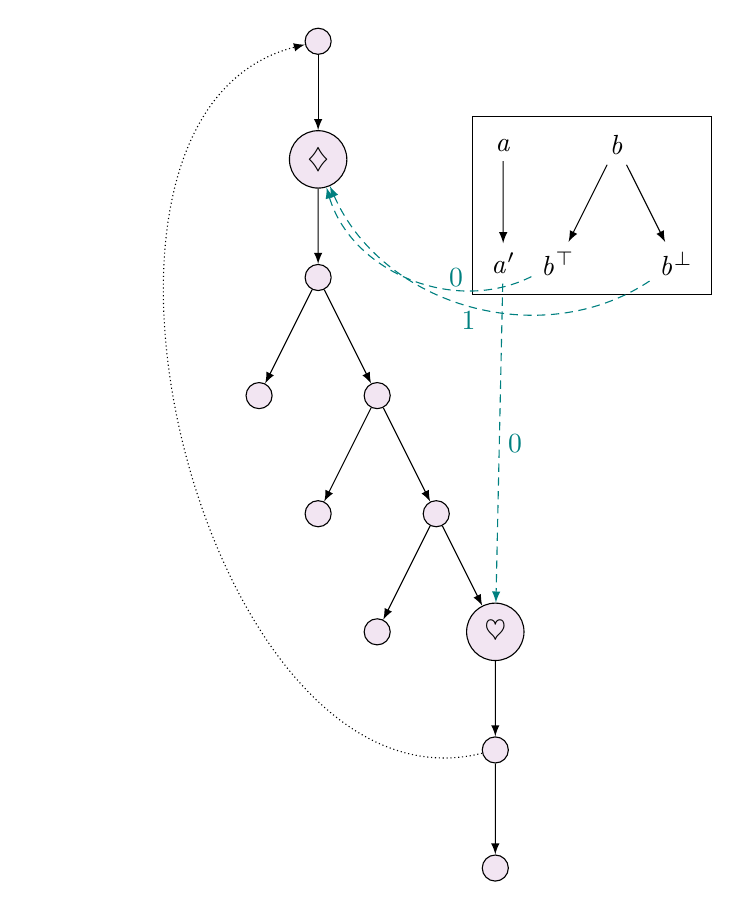
\begin{tikzpicture}[edge from parent/.style={draw,-latex}]
    \node[draw,circle,fill=violet!10] (circuit) {} child {
      node[draw,circle,fill=violet!10] (bmaker) {$\diamondsuit$}
      child {node[draw,circle,fill=violet!10] {}
        child {node[draw,circle,fill=violet!10] {}}
        child {node[draw,circle,fill=violet!10] {}
          child {node[draw,circle,fill=violet!10] {}}
          child {node[draw,circle,fill=violet!10] {}
            child {node[draw,circle,fill=violet!10] {}}
            child {node[draw,circle,fill=violet!10] (amaker) {$\heartsuit$}
              child {node[draw,circle,fill=violet!10] (ref) {}
                child {node[draw,circle,fill=violet!10] {}}
              }
            }
          }
        }
      }
    };
    \node[below right=1cm and 2cm of circuit] (a) {$a$} child {node (aprime) {$a'$}};
    \node[right=1 cm of a] (b) {$b$}
    child {node (btop) {$b^\top$}}
    child {node (bbot) {$b^\bot$}};
    \node[draw,fit=(a) (aprime) (b) (btop) (bbot)] {};
    \draw[-latex] (ref) edge[densely dotted,bend left=90] (circuit);
    \draw[-latex,color=teal] (aprime) edge[densely dashed] node[xshift=2mm,color=teal] {$0$} (amaker);
    \draw[-latex,color=teal] (btop) edge[bend left=50,densely dashed] node[xshift=6mm,color=teal] {$0$} (bmaker);
    \draw[-latex,color=teal] (bbot) edge[bend left=50,densely dashed] node[yshift=-2mm,color=teal] {$1$} (bmaker);
  \end{tikzpicture}
  \caption{A circuit (outside the box) and a forest of domains (inside the box). The dotted line on the left will be added if \texttt{identifyRecursion} returns a non-\texttt{null} mapping. The dashed edges with their labels represent the $\kappa$ function. The circuit nodes with symbols in them are the nodes that introduce new (sub)domains.}
  \label{fig:example}
\end{figure}

TODO: explain what the second return statement is about and why a third one is not necessary.

TODO: mention which one is the main function, what each function takes and returns.

\begin{example}
  TODO: explain how the algorithm establishes a recursive relationship from
  % 1. formulas (both the Forclift representation and the more normal way to write down the same thing)
  % 2. definitions of delta_c, delta_d, kappa, pi
  \begin{align*}
    \forall X \in a'. \forall Y \in b^\bot. \forall Z \in b^\bot. Z \ne Y &\implies \neg p(X, Y) \lor \neg p(X, Z) \\
    \forall X \in a'. \forall Y \in b^\bot. \forall Z \in a'. X \ne Z &\implies \neg p(X, Y) \lor \neg p(Z, Y)
  \end{align*}
  to
  \begin{align*}
    \forall X \in a. \forall Y \in b. \forall Z \in b. Y \ne Z &\implies \neg p(X, Y) \lor \neg p(X, Z) \\
    \forall X \in a. \forall Y \in b. \forall Z \in a. X \ne Z &\implies \neg p(X, Y) \lor \neg p(Z, Y)
  \end{align*}
  and mention \cref{fig:example}. Solution map (stored as the edge label):
  \begin{align*}
    \rho(a') &= (a, \{\, (\diamondsuit, 0) \,\}) \\
    \rho(b^\bot) &= (b, \{\, (\heartsuit, 1) \,\})
  \end{align*}
\end{example}

TODO: conclude with a description of the inference rule and the node/edge type.

\section{New Node Types}

\subsection{Improved Domain Recursion}

The original version of domain recursion is here \cite{DBLP:conf/nips/Broeck11}.

\subsection{Constraint Removal}

\section{Other Topics}

\begin{itemize}
\item domains, smoothing, and avoiding infinite cycles
\item new rules that don't create nodes (e.g., duplicate removal, unconditional contradiction detection, etc.)
\end{itemize}

\section{Circuit Evaluation}

TODO: new node types, their algebraic/graphical representation, what info they hold, and how they're created.

TODO: describe evaluation of: and, counting, constraint removal, ref, unit, contradiction, improved domain recursion. Most of this will be from \cite{DBLP:conf/ijcai/BroeckTMDR11}.

\bibliographystyle{acm}
\bibliography{notes}

\end{document}
